\documentclass{article}

\usepackage[a4paper, total={6in, 8in}]{geometry}
\usepackage{setspace}
\usepackage{lineno}
\usepackage[dvipsnames]{xcolor}
\usepackage{graphicx}
\usepackage{booktabs}
\usepackage[square,sort,comma,numbers]{natbib}
\setcitestyle{authoryear,open={(},close={)}}

\graphicspath{{figures/}}
    
\title{How does date-rounding affect phylodynamic inference for public health?}
\author{Leo A. Featherstone$^{\ast,1}$, Wytamma Wirth$^{1}$,Courtney Lane$^{1}$, Benjamin Howden$^{1}$,\\Danielle Ingle$^{1}$, Sebastian Duchene$^{1}$}

\begin{document}

\maketitle
\linenumbers
$^{1}$ Peter Doherty Institute for Infection and Immunity, University of Melbourne, Australia.\\
*email: leo.featherstone@unimelb.edu.au

\section*{Abstract}
 TODO: Leo to rewrite at end \\
 Despite its broad applicability, phylodynamic analyses always begin with pathogen genome sequences and associated sampling times. But, the release of sampling time data can pose a threat to patient confidentiality. In response, sampling times are often only given with reduced resolution to the month or year, but this can bias estimates and mislead the interpretation of results. Here, we characterise the extent to which reduced sampling time resolution can bias phylodynamic analyses across a diverse range of empirical and simulated datasets and offer a guideline on when date rounding biases phylodynamic inference. We also show that this bias is both unpredictable in its direction and compounds for increased evolutionary rates and decreased date-resolution. We conclude by suggesting a simple form of encryption where exact sampling times are essential and there is a clear risk to patient confidentiality.


\begin{spacing}{1.5}
\section*{Introduction}

Phylodynamics is commonly use to estimate the parameters of epidemiological spread from pathogen genome sequences. It offers valuable insight where the age, origin, and transmission is difficult to infer from other data. 


Pathogen genomics is playing an increasingly important role in our understanding of infectious outbreaks in recent decades. It offers insight across the scales of transmission from the pandemic and epidemimec scales, such as for SARS-CoV-2 and Ebola virususes, to more localised transmission or bacterial pathogens \citep{lancet2021genomic}. Phylodynamic analysis has consequently emerged as a key method to make temporal and spatial inference from pathogen genomes, particularly since the 2013-2016 West African Ebola outbreak \citep{mbala2019medical}. It is most useful where temporal and spatial records of transmission are sparse, because it allows genomic information help fill the gaps of traditional epidemiological data.

Phylodynamic methods offer a range of inferences from pathogen sequence data, including epidemioloigcal transmission and migration rates, pathogen population size, spatial dynamics, time and location of origin, and the identification of variants of concern \citep{featherstone2022epidemiological, attwood2022phylogenetic, du2015getting,volz_fitness_2023}. The basis of all such inferences is that epidemiological spread leaves a trace in the form of substitutions that can be used to reconstruct transmission processes. Pathogen populations that meet this assumption known as `measurably evolving populations' \citep{drummond2003measurably, biek_measurably_2015}. In accordance, phylodynamics always typically on a combination of genome sequence and associated sampling times to leverage measurable evolution and infer temporally explicit parameters of transmission and pathogen demography.

Ideal phylodynamic datasets should include precise sampling dates alongside genome sequences \citep{black2020ten}, but sampling times necessarily carry over information about times of hospitalisation, testing, or treatment than can be used to identify individual patients. This can pose an unacceptable risk for patient confidentiality. In some cases, sampling times or dates of admission that are even available for purchase have allowed identification for a majority of patients on record \citep{sweeney_matching_2013,shean_private_2018}. In acknowledgement of this risk, \citet{shean_private_2018} suggest that Expert Determination govern whether sampling times be released alongside genome sequences, and the resolution to which they are disclosed (day, month, year). Essentially, This process involves an expert opinion on whether information is safe to release on a dataset-by-dataset basis.

From a phylodynamic point of view, sampling times with reduced resolution are usable. In principle, uncertainty in sampling times can be modelled, using Bayesian inference \citep{shapiro2011bayesian}, but such an approach is effective when samples with uncertain dates are a small proportion of the data set \citep{rieux2017tipdatingbeast}.

The most common technique for using imprecise sampling times requires the researcher to assume that they have been sampled at an arbitrary day. Selecting the arbitrary day can be motivated by convenience, such as all samples from 2020 being assigned 1st January 2020 or 15 June 2020, or by sampling a random day within 2020 using a statistical distribution for each sample. In either case, both approaches introduce a degree of error. Moreover, theoretical and applied results show sampling times can substantially direct inference \citep{featherstone_decoding_2023,featherstone_infectious_2021,volz_sampling_2014}, raising the question of whether reduced date resolution biases inference. This question has practical significance, as there are many examples of phylodynamic analysis conducted for a diverse array of viral and bacterial pathogens with reduced date resolution. These include viral pathogens such as Rabies Virus, Enterovirus, SARS-CoV-2, Dengue virus \citep{talbi_phylodynamics_2010,xiao_genomic_2022,wolf_temporal_2022,bennett_epidemic_2010}, and bacterial pathogens such as \textit{Klebsiella pneumoniae}, \textit{Streptococcus pneumoniae}, and \textit{Mycobacterium tuberculosis} \citep{cella_multi-drug_2017,azarian_impact_2018,merker_evolutionary_2015}. 

The degree of precision in collection times is also relevant for database design and curation because sampling dates are often considered part of the associated metadata and may be unavailable or imprecise due to inconsistencies between between storage platforms \citep{raza2016big}. For example, as of early August 2023, there were roughly 15.8M SARS-CoV-2 genome sequences available on GISAID with 2.4\% (382K) of these having `incomplete' date information, where sampling dates are absent or only given to the year. In other words, roughly 1 in 50 sequences lacked clear date resolution, reflecting global inconsistency in sampling times records.

In acknowledgment of this issue, we characterised when and how biases arise from reduced date resolution in phylodynamic inference. We analysed four empirical datasets of SARS-CoV-2, H1N1 Influenza, \textit{M. tuberculosis}, and \textit{Shigella sonnei} and conducted a simulation study with conditions that correspond to parameter estimates from each. These pathogens have undergone substantial genome surveillance and have different infectious periods and molecular evolutionary dynamics, thus providing a diverse representation of phylodynamics' applicability. For each empirical and simulated dataset, we repeated analyses with sampling times rounded to the day, month, or year and studied the resulting bias in inferred parameters. For example, 2021/10/11 would be specified as 2021/10/01 when the day is not provided (and arbitrarily set to the first of the month) and 2021/01/01 when the month are day are not provided (and arbitrarily set to the first day of the first month.

We focused on inference of the reproductive number ($R_0$ or $R_e$), defined as the average number of secondary infections stemming from an individual case, the age of each outbreak, and the evolutionary rate (substitutions per site per year) in each dataset. Together, these parameters span much of the insight that phylodynamics offers through inferring when an outbreak started and how fast it proceeded. The evolutionary rate is also the central parameter relating evolutionary time to epidemiological time, so any resulting bias has a pervasive effect throughout a phylodynamic model.

 We show that reduced date resolution causes bias that compounds where the temporal resolution that is lost exceeds the average time required for a mutation to arise in a given pathogen. We visualise the relationship between date resolution and average mutation time in Fig \ref{fig:plane}. For example, H1N1 influenza virus accumulates substitutions at a rate of about 4 $\times10^{-3}$ subs/site/year \citep{hedge_2013_real-time}. With a genome length of 13,158bp, we then expect a substitution to accrue roughly every week. Therefore, rounding dates to the month or year will conflate the times over which substitutions arise and bias the resulting inferences. Our results demonstrate this effect and furthermore show that it is exacerbated with increased degree of rounding.
 
 In contrast, the evolutionary rate for \textit{M. tuberculosis} has been estimated to be of the order of $10^{-8}$ subs/site/year \citep{menardo2019molecular}, resulting in about one substitution every 23 years. For this bacterium, we find that providing the sampling year or month is be sufficiently precise to correctly inform phylodynamic analyses. The SARS-CoV-2 and \textit{S. sonnei} dataset, which accrue mutations at a rate intermediate to these two examples accordingly shows intermediate levels of bias with date rounding. Similarly \textit{S. sonnei} accrues mutations between the order of months and years, so bias is introduced when rounding dates to the year.

 However, bias does not always move in the same direction. Rounding can interact with the sampling time distribution to more evenly disperse mutations such that rates can be deflated. Taken together, we find that reduced date resolution biases estimates, and that this bias is not predictable, as it is affected by sampling time distribution as well as evolutionary rates. Finally, we conclude that where date rounding poses can mislead inferences, we propose a simple form of encryption whereby on a dataset-by-dataset basis, all sampling dates are be shifted by a random number, such that inference is preserved but precise times are unavailable to identify patients.

\begin{figure}[!h]
    \centering
    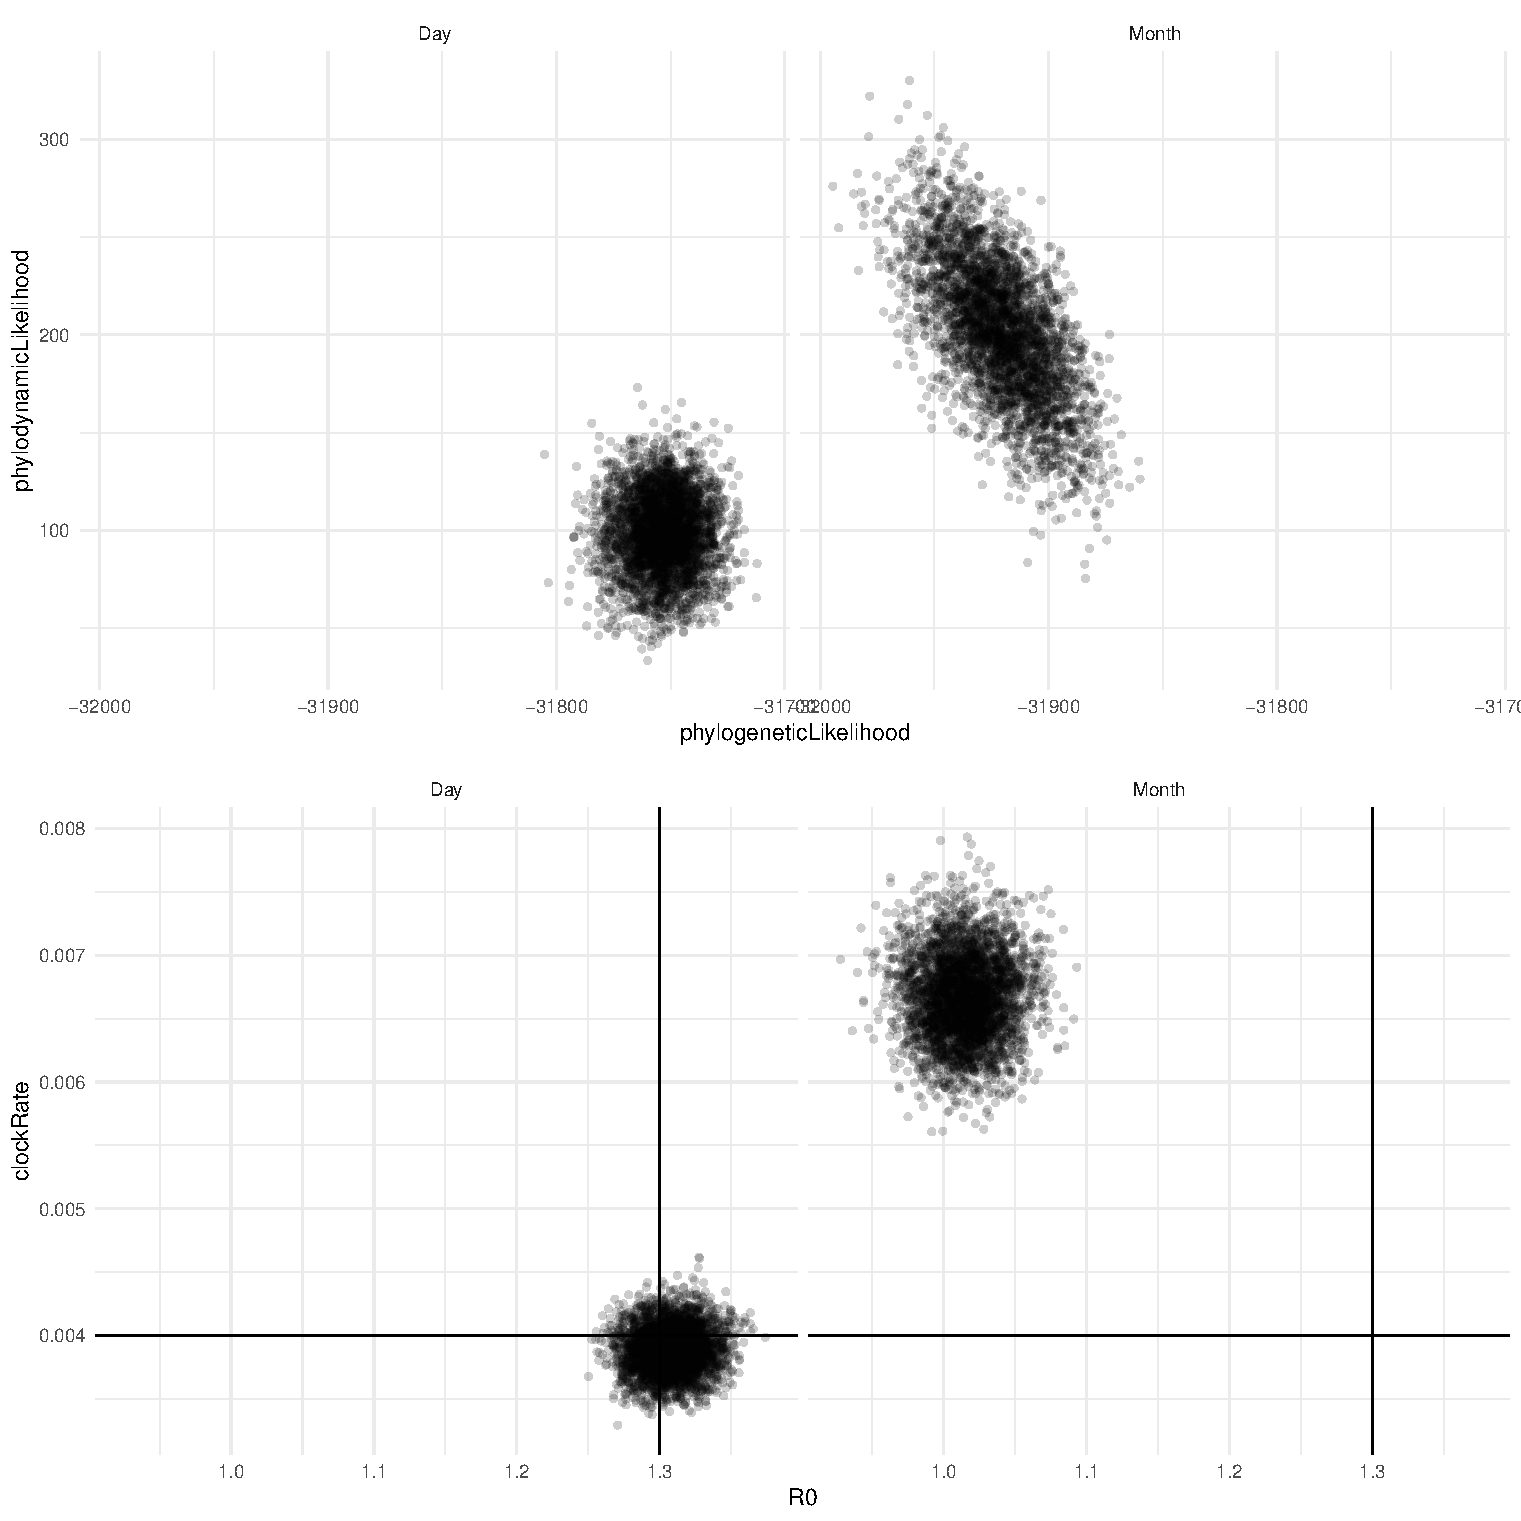
\includegraphics[width = 0.5\textwidth]{plane.pdf}
    \caption{The average time to accrue one mutation based on a fixed genome size and evolutionary rate ($\frac{\textnormal{Genome Length}}{\textnormal{Evolutionary rate (subs/site/time)}}$) against the temporal resolution lost by date rounding. We hypothesised and showed that when analyses for a given pathogen round dates to an extent nearing or crossing the diagonal from left to right, biases is induced in $R_e$, age of the outbreak, and evolutionary rate. Mutation rates are taken from each source for the empirical data. We do not report the numerical axis as this figure is designed to illustrate a concept rather than serve as a reference, in the same spirit as is inspiration in Figure 2 of \citet{biek_measurably_2015}.}
    \label{fig:plane}
\end{figure}


\section*{Methods}
\subsection*{Overview}
Our study is based on 4 empirical datasets of H1N1 influenza virus, SARS-CoV-2, \textit{Staphylococcus aureus}, and \textit{Mycobacterium tuberculosis}. We also conducted a  simulation study with parameters tailored for each dataset. These data were chosen to capture span the usual parameter space for substitution rate and sampling duration in phylodynamics for epidemiology (roughly $10^{-3}\textnormal{-to-}10^{-8}$ (subs/site/yr) for substitution rate and Months-to-Decades for duration of sampling).

To assess the effects of date rounding, we conducted phylodynamic analyses for both the empirical and simulated datasets with sampling dates rounded to the day, month, or year. For example, two samples from 2000/05/29 and 2000/05/02 would become 2000/05/15, if rounded to the month. We then measured the resulting bias in epidemiologically- or phylodynamically-important parameters: the reproductive number ($R_0$ or $R_e$), substitution rate (subs/site/year), and the age of the outbreak (time to most recent common ancestor, tMRCA hereon). 

In this context $R_0$ refers to the \textit{basic} reproductive number and $R_e$ is the \textit{effective} reproductive number. These parameters correspond to the average number of secondary infections at the start of an outbreak (i.e. assuming a fully susceptible population; $R_0$) or thereafter ($R_e$) (reviewed by \citep{featherstone2022epidemiological, du2015getting, kuhnert2011phylogenetic}). We consider the age of outbreaks as the tMRCA to facilitate comparison between phylodynamic models because some analyses include the length of the root branch in the age of the outbreak \citep{stadler2012estimating}.

The two viral datasets consist of samples from the 2009 H1N1 pandemic (n=161) from \citet{hedge_2013_real-time}, and a cluster of early SARS-CoV-2 cases from  Victoria, Australia in 2020 (n = 112) \citep{lane2021genomics}. The bacterial datasets consist \textit{S. aureus} 104 samples from New-York sampled over ~2 years \citet{duchene_2016_genome,volz_modeling_2018,uhlemann_molecular_2014}, and 30 \textit{M. tuberculosis} samples from a ~25 year outbreak studied by \citet{kuhnert_tuberculosis_2018}. These data were chosen because they encompass a diversity of epidemiological dynamics, timescales, and variable rates of substitution.

\subsection*{Simulation Study}

\begin{table}[h!]
    \centering
    \caption{Parameter sets outbreaks corresponding to each empirical dataset.}
    \begin{tabular}{l|c|c|c|c|c|c|l|}
    \hline
    Microbe                     &   $\delta (yrs)^{-1}$    & $R_0$ &   $R_{e_1}$   &  $R_{e_2}$    &   $p$   &   $T$(yrs)   & Source \\
    \hline
    H1N1                        &   91.31    & 1.3 &   -   &  -    &   0.015   &   0.25 & \citet{hedge_2013_real-time} \\
    SARS-CoV-2                  &   36.56    & 2.5 &   -   &  -   &   0.80   &  0.16 & \citet{lane2021genomics} \\
    \textit{S. aureus}    &   0.93    &  - &   2.0   &  1.0   &   0.2$^{\dagger}$   &   25 & \citet{duchene_2016_genome} \\
    \textit{M. tuberculosis}    &   0.125    &  - &   2.0   &  1.10    &   0.08   &   25.0 & \citet{kuhnert_tuberculosis_2018} \\
    \hline
    \end{tabular}
    \label{tab:sim_parms}
\end{table}
\footnotesize{$^\dagger$ $p$ was set to zero before $T=22$}

We simulated outbreaks as birth-death sampling processes using the ReMaster package in BEAST v2.7.6 \citep{vaughan_remaster_2024,bouckaert_beast_2019}. Simulations consisted of 4 parameter settings corresponding to each empirical dataset (Table \ref{fig:emp-parm}), with 100 replicates over each. All parameter sets include a proportion of sequenced cases ($p$), outbreak duration ($T$), and a "becoming un-infectious" rate ($\delta$ = reciprocal of the duration of infection). For simulations corresponding the viral datasets, transmission is modelled via $R_0$, the average number of secondary infections (assuming a fully susceptible population). For those corresponding to the bacterial datasets, we allow the effective reproductive numbers to vary over two intervals ($R_{e_1}$ and $R_{e_2}$ respectively). For the \textit{S. aureus} setting, the change time was at $t=22$ with the sequencing proportion ($p$) also set to zero before this time to replicate the sampling effort generating the dataset. For the \textit{M. tuberculosis} dataset, the change time was fixed at halfway through simulations ($t=12.5$) with one sequencing proportion throughout.

\begin{table}[h!]
    \centering
    \caption{Substitution rates and genome length for sequence simulation.}
    \begin{tabular}{l|c|l|l}
    \hline
    Microbe                     &   Substitution Rate (subs/site/yr) & Genome Length & Time/Sub/Genome (yrs)  \\
    \hline
    H1N1                        & $4\times10^{-3}$ & 13158 & 0.0190\\
    SARS-CoV-2                  & $1\times10^{-3}$ & 29903 & 0.0334\\
    \textit{S. aureus}    & $1\times10^{-6}$ & 2900000  & 0.3458\\
    \textit{M. tuberculosis}    &   $1\times10^{-7}$ & 4300000 & 2.3256\\
    \hline
    \end{tabular}
    \label{tab:seq_parms}
\end{table}

Overall, simulations yielded a total of 400 outbreaks which we then used to simulate sequences data under a Jukes-Cantor model using Seq-Gen v1.3.4 \citep{rambaut_seq-gen_1997} with fixed substitution rates (Table \ref{tab:seq_parms}). We chose a simple substitution model to reduce parameter space and because substitution model mismatch has been widely explored elsewhere \citep{lemmon2004importance}.

We then analysed each of the 400 simulated datasets under each of the 3 date treatments (Day, Month, and Year resolution) and yielding 1800 analyses (1200 under birth death and 600 under coalescent exponential tree-priors). We used identical model specifications and prior setting as for the corresponding empirical datasets. We ran each MCMC chain for $5\times18^{8}$ steps, sampling every $10^{4\textnormal{th}}$ step and discarding the first 50\% as burnin. We then discarded all analyses that did not have $ESS\geq200$, leaving a total of 1670 joint posteriors.

\subsection*{Empirical Data}
We conducted Bayesian phylodynamic analyses using a birth-death skyline tree-prior in BEAST v2.7.6 for all datasets \citep{bouckaert_beast_2019,stadler2012estimating}. We also fit a coalescent exponential tree-prior for the viral datasets \citep{kingman_1982_coalescent}. We sampled from the posterior distribution using Markov chain Monte Carlo (MCMC), with $5\times10^{7}$ steps ($1\times10^{7}$ for SARS-CoV-2 data) sampled every $10^{4}$, and the initial 10\% discarded as burnin. We assessed convergence by ensuring $ESS\geq200$ for all parameters and likelihoods.

\subsubsection*{H1N1}
The H1N1 data consist of 161 samples from North America during the 2009 H1N1 influenza virus pandemic, analysed by \citet{hedge_2013_real-time}. Samples originate from April to September 2009 and provides an example of a rapidly evolving pathogen sparsely sampled during an emerging outbreak. 

We placed a $\textnormal{Lognormal}(\mu=0,\sigma=1)$ prior on $R_0$, $\beta(1,1)$ prior on $p$, and fixed the becoming-uninfectious ($\delta = 91$), corresponding to a 4 day duration of infection. We also placed an improper ($U(0,\infty)$) prior on the origin and a $U(10^{-4},10^{-2})$ prior on the substitution rate. This prior corresponds to analysis of these data in \citet{featherstone_decoding_2023}.

\subsubsection*{SARS-CoV-2}
The SARS-CoV-2 data are 112 samples from a densely sequenced transmission cluster in Victoria, Australia in from late July to mid September 2020 \citet{lane2021genomics}. These data are similar to the H1N1 datasets in presenting a quickly evolving viral pathogen, but contrast in that virtually all cases in the cluster were sequenced. 

Prior configurations are identical to those used in \citet{featherstone_decoding_2023} to analyse the same data. Briefly, we placed a $\textrm{Lognormal}(\textrm{mean}=1, \textrm{sd}=1.25)$ prior on $R_0$ and an $\textrm{Inv-Gamma}(\alpha=5.807, \beta=346.020)$ prior on the becoming-uninfectious rate ($\delta$).  The sampling proportion was fixed to $p=0.8$ since every known Victorian SARS-CoV-2 case was sequenced at this stage of the pandemic, with a roughly 20\% sequencing failure rate. We also placed an $\textrm{Exp}(\textrm{mean}=0.019)$ prior on the origin, corresponding to a lag of up to one week  between the index case and the first putative transmission event. The substitution rate was fixed a $10^{-3}$ following \citep{duchene_temporal_2020}.

\subsubsection*{\textit{Staphylococcus aureus}}
The \textit{S. aureus} dataset originates from \citet{uhlemann_molecular_2014} and we analysed a subset of the data later considered in \citet{duchene_2016_genome} and \citet{volz_modeling_2018}. It consists of a single nucleotide polymorphism (SNP) alignment of 104 sequenced isolates sampled in New York from 2009 to 2011. Populations growth is understood to have been driven by $\beta$-lactam use beginning in the 1980s. These data therefore provide a comparison to the \textit{M. tuberculosis} dataset in a shorter sampling span from am outbreak of similar duration.

To accommodate changing transmission dynamics, we included two intervals for $R_e$ with a $\textnormal{Lognormal}(\mu=0,\sigma=1)$ prior on each. We also placed a $\beta(1,1)$ prior on the sampling proportion, which was otherwise fixed to 0 before the first sample to capture the lag in sampling. We also placed a $U(0,1000)$ prior on the origin, and fixed the becoming un-infectious rate at $\delta=0.93$, corresponding to a nearly year-long duration of infection following \citet{volz_modeling_2018}.

\subsubsection*{\textit{Mycobacterium tuberculosis}}
The \textit{M. tuberculosis} dataset consists of 36 sequenced isolates from a retrospectively recognised outbreak in California, USA, that originated in the Wat Tham Krabok refugee camp in Thailand and was originally studied in \citet{kuhnert_tuberculosis_2018}. We applied the same prior configurations as \citet{kuhnert_tuberculosis_2018}, with the exception of including 2 intervals for $R_e$ and fitting a strict molecular clock with a $\Gamma(\alpha=0.001,\beta=1000.0)$ prior.

\section*{Results}
\subsection*{Simulation study}
The viral simulation conditions (SARS-CoV-2 and H1N1) display the greatest bias in mean posterior estimates of substitution rate, outbreak age, and reproductive number with decreasing date resolution (Figure \ref{fig:sim-parms} A-C). In the bacterial simulation conditions exhibit a lesser bias in response to decreasing date resolution. The \textit{M. tuberculosis} simulation conditions is effectively inert to decreasing date resolution down to the year with mean posterior estimates for each parameter of interest remaining consistent across date resolution. The \textit{S. aureus} provides an important intermediate case where estimates of each parameter changing when transitioning from Month to Year date resolution (see crossing of lines from Month to Date resolution in the \textit{S. aureus} column of Figure \ref{fig:sim-parms}). These trends generally support the hypothesis of decreasing date resolution causing increased bias where the lost resolution exceeds the average time for a substitution to arise. In this case, date rounding compresses divergent sequences in time, driving a signal for higher rates of evolution and transmission locally to each cluster of sampling times.  The effect is less pronounced in the bacterial conditions where the date resolution lost is a smaller fraction of the effective substitution time, such as for the \textit{M. tuberculosis} and \textit{S. aureus} conditions.  However, there are also notable deviations in the this effect bias across duration of sampling efforts, tree priors, and simulation conditions.

\begin{figure}
    \centering
    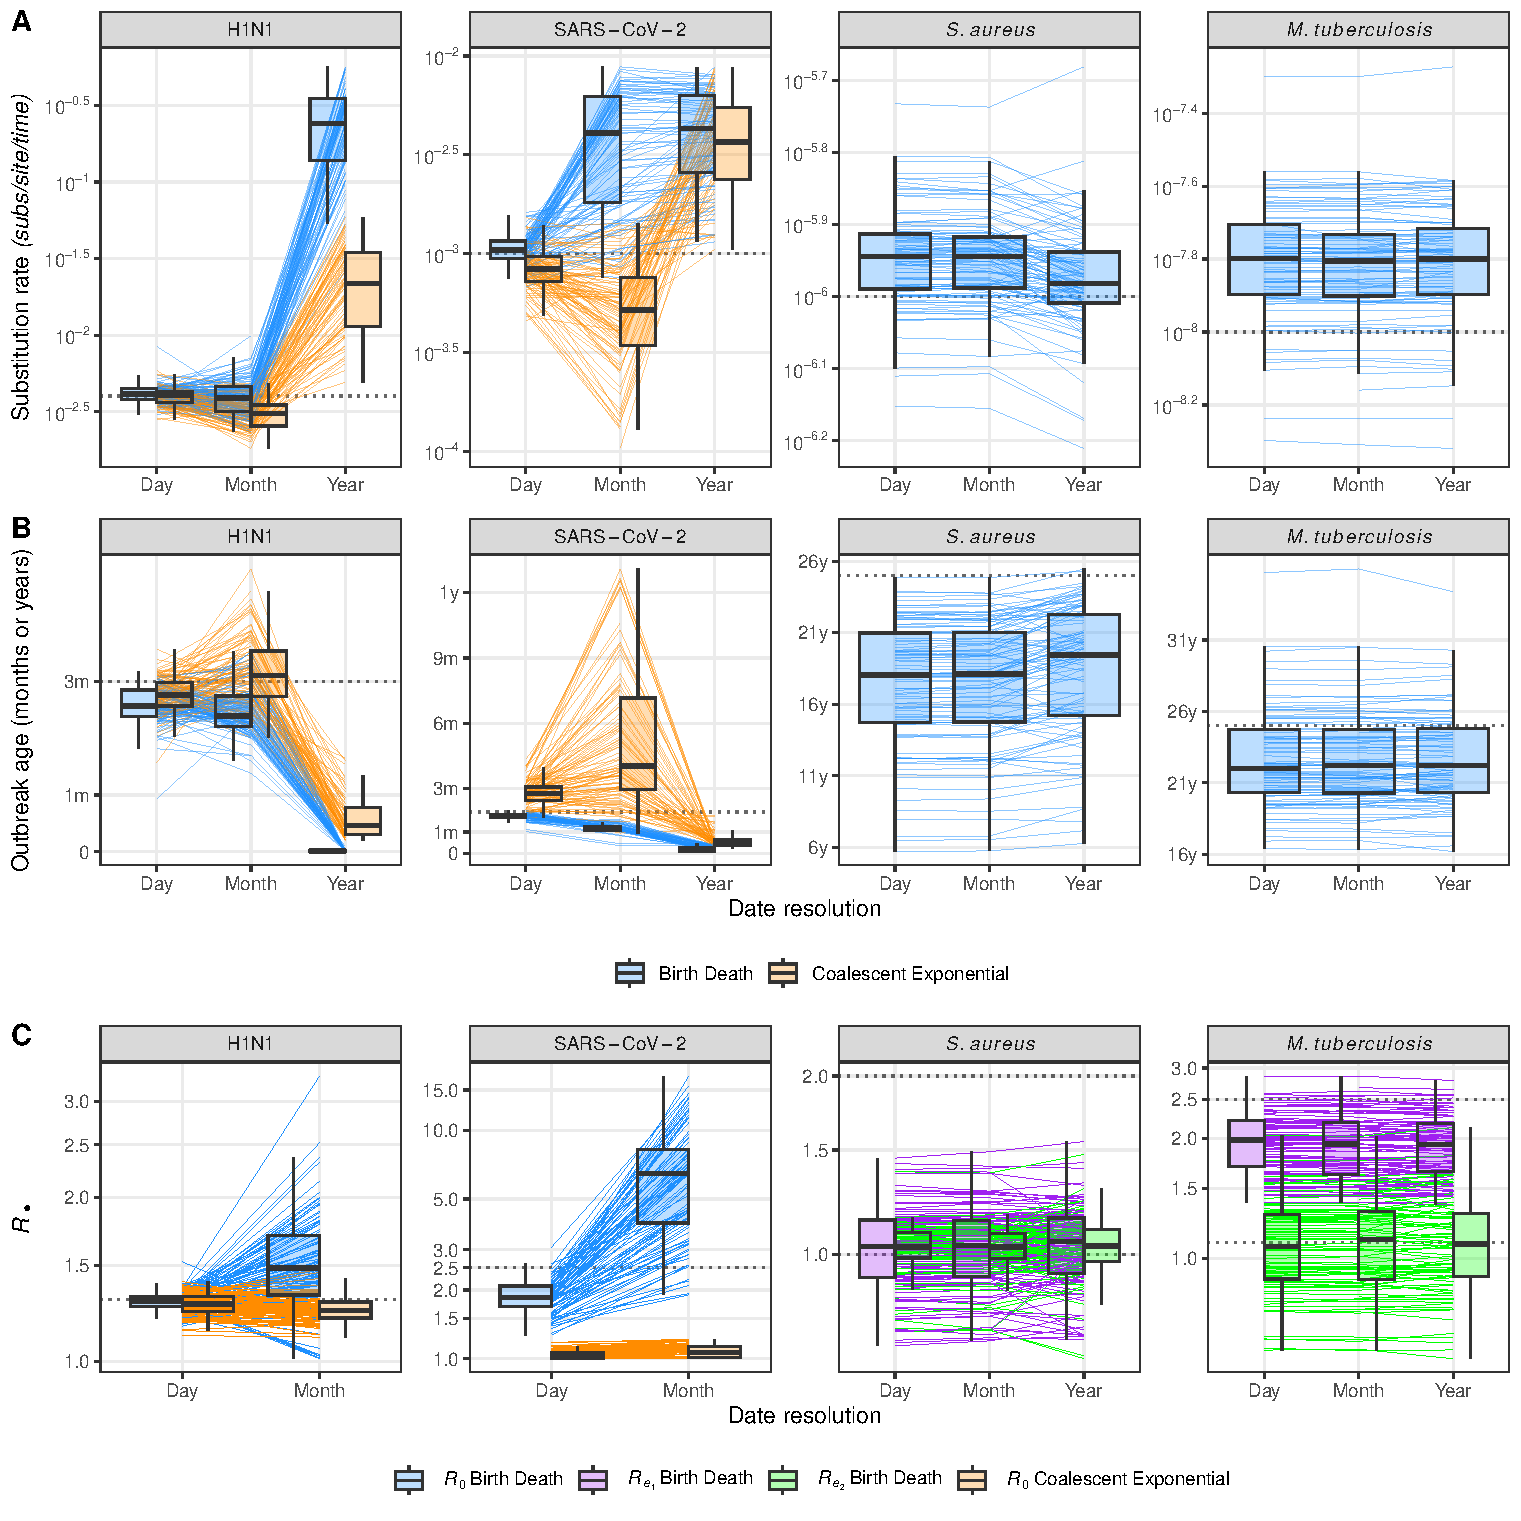
\includegraphics[width=\textwidth]{simulation_parm_panel.pdf}
    \caption{Mean posterior estimates for parameters of interest for each simulated dataset varying across date resolution. Individual lines track inference for one simulated dataset over decreasing date resolution while boxplots are given to summarise the spread and direction of bias across simulated datasets. Rows correspond to individual parameters, columns correspond to simulation condition (underlying parameters corresponding to each pathogen dataset), and colour corresponds to tree prior or reproductive number interval. Dashed horizontal lines correspond to the true value under which each dataset was simulated. In general, reduced date resolution leads to bias where resolution is greater than the average time until mutation.  (\textbf{A}) Inferred mutation rate across simulation scenarios. (\textbf{B}) Inferred age of outbreaks. (\textbf{C}) Inferred reproductive number. }
    \label{fig:sim-parms}
\end{figure}

For the viral simulation conditions, there is an upwards bias in mean posterior reproductive number and substitution rate with decreasing date resolution for the viral simulation conditions. At the same time, the mean posterior age of each outbreak decreases in relation with increased rates of substitution (Figure \ref{fig:sim-parms} A-C). The coalescent exponential shows overall downwards bias in the substitution rate for the SARS-CoV-2 and H1N1 treatments at month resolution while the birth-death exhibits upwards bias. Since the sampling times for each viral dataset are distributed over 3 months, date rounding will compress the diversity among samples within each month, but also increase the distance in time between months, driving a signal for lower transmission and substitution rates over this time. The different phylodynamic likelihood functions for each tree prior appear to respond to this warped distribution of diversity over time with the coalescent exponential placing more weight on decreased rates of evolution while the birth death places more on increased substitution rates. At Year-resolution there is there is also lower bias in estimates of substitution rate for the coalescent exponential, however both models prefer upwards biased substitution rates as Year resolution. This is probably because Year resolution clusters all sampling times to one time point, meaning an inflated rate of substitution is needed to model the burst in diversity at one time point relative to the start of each outbreak (Figure \ref{fig:densitree}). At the same time, the mean posterior age of each outbreak moves inversely to bias in the substitution rate. This is the result of a well understood axis among phylodynamic models where higher rates of evolution suggest shorter periods of evolution \citep{featherstone_decoding_2023}.

The reproductive number for each viral dataset ($R_0$) also becomes biased with decreasing date resolution under the birth death. This is in agreement with temporal clustering of samples driving a signal for higher transmission rates. Conversely, estimates under the coalescent exponential remain largely unchanged at Month-resolution. This is probably because the model can adjust the population size parameter instead of modulating the growth rate, which would be reflected in $R_0$. Estimates of $R_0$ for the SARS-CoV-2 condition are also biased heavily downwards, and this is probably due to high sequencing proportions violating the assumption of low sampling under the coalescent.

The \textit{S. aureus} condition yields consistent estimates of substitution rate, outbreak age, and reproductive number ($R_e$ in this case) when dates are rounded to the month (Figure \ref{fig:sim-parms} \textit{S. aureus} column). At year resolution the posterior substitution rate appears appears biased downwards. This can be explained by the two year sampling duration of the \textit{S. aureus} condition, such that samples rounded to the year will be on average further apart in time than if dates are given to the month or day (Figure \ref{fig:densitree}). This spacing of diversity in time likely drives the signal for lower substitution rates and an older outbreak in turn. There is no clear pattern in the direction of bias for $R_{e_1}$ and $R_{e_2}$ at year resolution, though estimates do deviate from those at month and day resolution. Estimates for $R_{e_1}$ are also overall lower than their true value of 2, but this is attributable to inconsistent sampling over the duration of the outbreak which has been shown previously for similar datasets in \cite{featherstone_infectious_2021}.

The \textit{M. tuberculosis} simulation conditions effectively act as a control conditions, since it appears inter to date rounding. Again this is expected, because this dataset reflects both longer simulation time, with temporal clustering less likely to inflate $R_e$, but also the effective mutation time is longer than 1 year. As such, even rounding to a year is unlikely to drive a signal for increased evolutionary rate or a more recent origin time.

Phylodynamic and phylodynamic likelihoods also vary with decreasing date resolution (Figure \ref{fig:sim-likeihood}). Variation also increases with lesser date resolution between Month and Year. This shows that altered date resolution affects the likelihood manifold of each analysis.

\subsection*{Empirical Results}

Broadly, analyses of the empirical datasets reproduce the trends of bias in reproductive number, substitution rate, and time of origin from the simulation study (figures \ref{fig:empR},\ref{fig:empClock}). That is, the reproductive number increases with decreasing date resolution along with an increase in the substitution rate and corresponding decrease in the origin. There are a few exceptions to this trend that we consider below and which we attribute to the difference between simulated and empirical sampling time distributions.


\subsubsection*{H1N1 influenza virus}
Posterior $R_0$ increases with decreasing date resolution in a comparable way to the simulation study. However, the posterior substitution rate and origin time estimates remain essentially the same for day and month resolution (mean values of 1.083, 1.44 and $10^{-2}$, $10^{-2}$ respectively)(table \ref{table:empData}),  before moving upwards at year resolution as expected from the simulation study. This finding can be explained by the sampling time distribution, since the earlier samples occur later in their month (change fig3 to date axis proper), such that rounding them down to the first of the month effectively expands the timespan of sampling and thus driving signal for a lower evolutionary rate and older origin time.

\subsubsection*{SARS-CoV-2}
The SARS-CoV-2 datasets behaves as expected with respect to the posterior $R_0$. In particular, rounding to the month results in an unlikely, but plausible value of $R_0 = 5.972$ (table \ref{table:empData}). Rounding to the year inflates $R_0$ further as expected.

The posterior substitution rate of SARS-CoV-2 remains essentially stable when rounding to the month or year, with a mean value of $10^{-3.5}$ (subs/site/time) for both (table \ref{table:empData}). In addition, the origin time at month resolution becomes older after rounding the sampling times. These findings stand in contrast to the expectation of rounding sampling times leading to an overestimate of the substitution rate and a corresponding underestimation of the time of origin. We again attribute these differences to the distribution of the empirical sampling times, which are not as consistently distributed as they are for the simulated outbreaks. There appears to be one early sample (Fig \ref{fig:empR} A) that likely drives the signal for an older outbreak when rounding to the month because it is pushed back in time. At the same time, the substitution rate increases with decreasing date resolution as expected, likely due to the clustering of the the rest of the samples after the earliest.

\subsubsection*{\textit{S. sonnei}}
For $R_{e_1}$, the \textit{S. sonnei} dataset matched the simulation study, with month rounding having a minimal effect, but year rounding inducing an upwards bias (mean values of 1.072, 1.073 respectively, figure \ref{fig:empR}). $R_{e_2}$ departs from expectation. The estimate for this parameter decreases when rounding to the year. We speculate that this occurs because it compensates for elevated $R_{e_1}$ earlier in the outbreak. This is supported by a markedly lower origin value (mean of 4.004, table \ref{table:empData}), such that the outbreak appears as an intensified early burst. The substitution rate remains stable across date resolutions, which is expected given the overall low substitution in this data set (around $10^{-6}$ subs/site/year).

\subsubsection*{\textit{M. tuberculosis}}
The \textit{M. tuberculosis} data recapitulate the outcome of the simulation study. Posterior origin times and evolutionary rate remain consistent across decreasing date resolution at 20 years and $10^{-7}$ (subs/site/time) respectively. We observe minimal upwards bias in posterior $R_{e_1}$ and $R_{e_2}$, and the expectation that $R_{e_1} > R_{e_s}$ is met, coinciding with an earlier burst of transmission in agreement with \citet{kuhnert_tuberculosis_2018}. This reaffirms that if the effective mutation time sufficiently large compared to the date resolution lost, then date rounding has a lesser effect.

\begin{figure}[h!]
    \centering
    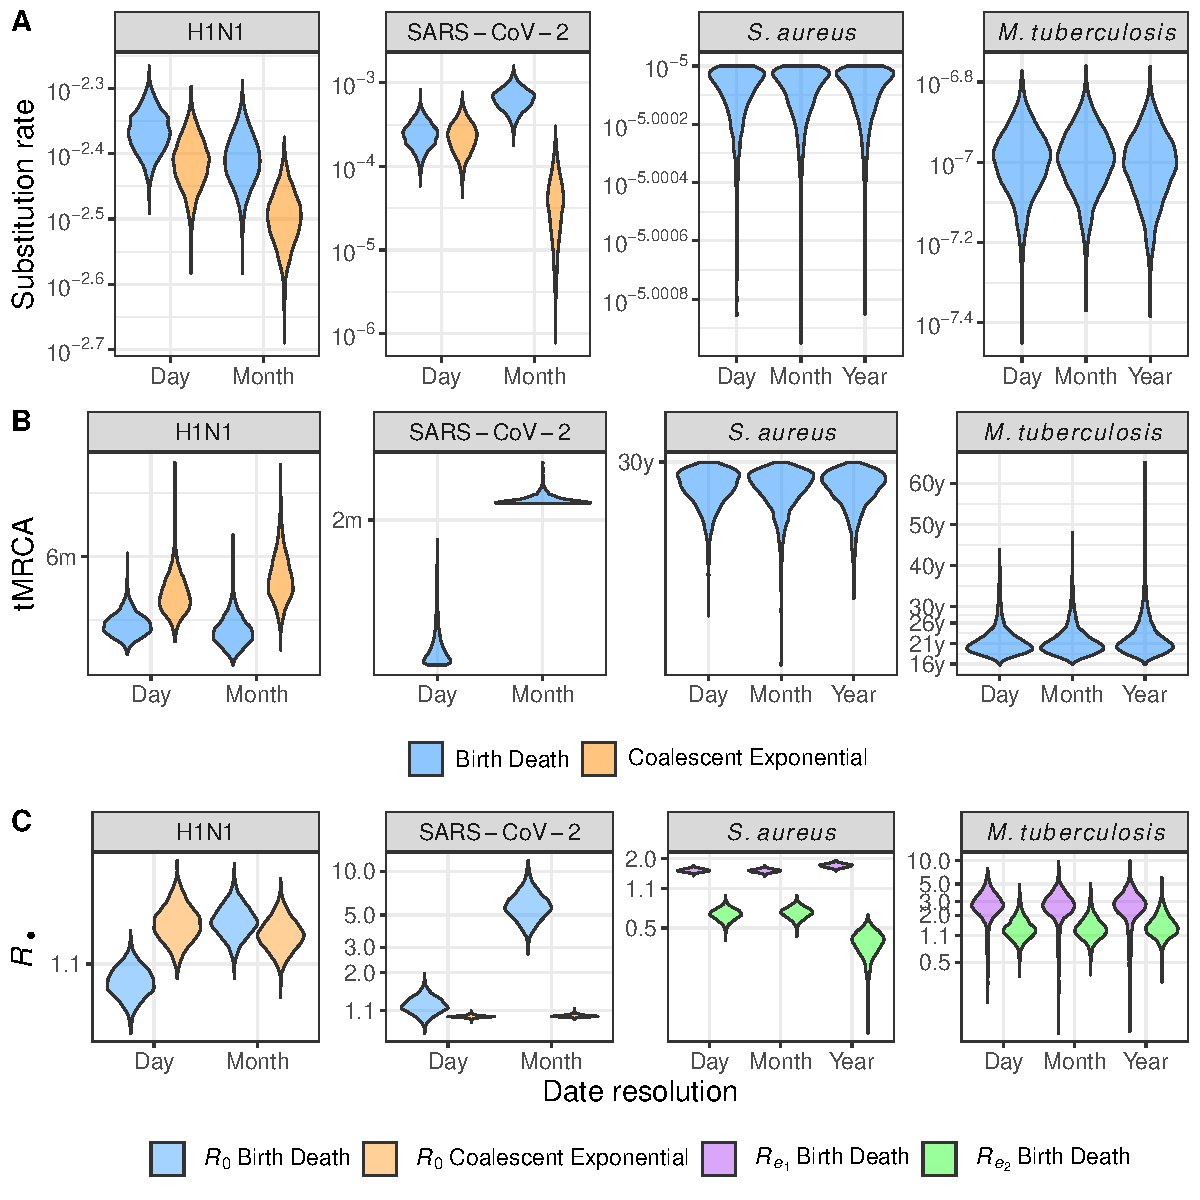
\includegraphics[width=\textwidth]{empirical_parms.pdf}
    \caption{Posterior distributions for parameters of interest estimated for each empirical dataset. Date resolution is given on the horizontal axis and colour denotes tree-prior. across date resolutions and tree-priors. Estimates at year-resolution are omitted because results deviate by many orders of magnitude due to sampling times being identical. (\textbf{A}) Posterior substitution rate across date resolutions. (\textbf{B}) Posterior outbreak age (tMRCA) on a month or year axis.  (\textbf{C}) Posterior reproductive number on a log-transformed axis.}
    \label{fig:emp-parm}
\end{figure}

\section*{Discussion}

The results of the simulation study can by summarised as showing that date rounding inflates estimates of evolutionary and epidemiological rates by temporally clustering differentiated genome sequences. This factor manifested as upwards bias of the effective reproductive number, substitution rate, and an underestimate of the age of the outbreak. The extent of the bias increased with more diverged sequences and decreased date resolution. In other words, it increases with the assertion that more evolution occurred in less time. This is why bias increased for simulation conditions with the highest amount of mutation per unit time - the H1N1 influenza virus conditions followed SARS-CoV-2 and \textit{S. sonnei}. Our \textit{M. tuberculosis} simulations, in their inertness to date rounding, also support this explanation because they were unlikely to generate any mutations over the month or even year mutation timescales.

Our empirical analyses broadly recapitulated the results of the simulation study, but also introduced notable exceptions which emphasised the unpredictability of the magnitude and direction of estimation bias when rounding dates. For example, the posterior substitution rate of the H1N1 influenza virus dataset did not display an upward bias when rounding to the month. The SARS-CoV evolutionary rate did not increase when moving from month to year rounding, and the posterior $R_{e_2}$ decreased when rounding to the year for the \textit{S. sonnei} dataset. In each case, we attribute these differences to the way in which the distribution of empirical sampling times differed from the consistency our our simulations. This meant that date rounding did not always result in temporal clustering of divergent sequences. In the example of the SARS-CoV-2 dataset where samples originated from the end of one month and start of the next, rounding down to the start of each month serves to spread out the samples over time, overriding the effect of clustering samples from the same month.

Taken together, the results form the simulation study and empirical data show that although date rounding biases empidemiological estimates in a theoretically predictable direction, the intensity of the bias is difficult to predict and varies with the parameter space the data notionally inhabit. Moreover, features of real-world sampling such as fine-scale clustering of sampling times over longer sampling efforts can unpredictably dampen or reverse expected bias due to date rounding. Put succinctly, date rounding induces bias unpredicable bias due to the interaction of theoretical aspects of phylodynamic models real-world data features.

We conclude that accurate sampling time information is essential where phylodynamic insight is needed to understand infectious disease epidemiology and evolution. There does not appear to be an clear way to adjust for the bias caused otherwise. However, as acknowledged from the beginning of this article, it may impose an unacceptable level of risk to patient confidentiality to release highly precise isolate sampling times, as can theoretically be used to identify individual patients. To circumvent this and deliver timely phylodynamic results, we finish by proposing an extremely simple form of encryption that may lower the level of risk in sharing sampling time to the day to acceptable levels.

\subsection*{The simplest encryption of dates}
The functional component of phylodynamic data is the \emph{difference} between sequences and dates, rather than their absolute values. After all, our methods are comparative within a sample. Thus we can prioritise exact information and protect patient identity at the same time. We propose that data deposited in online databases include dates that are all shifted in time by an unknown seed number, and reinterpret results by factoring this in. For example, if the sampling times of a dataset of 3 samples are 2000, 2001 and 2002, then we may randomly draw a seed of 1000 with which to shift and dates deposit online 2000, 2001 and 2002 $\rightarrow$ 3000, 3001 and 3002. Then results can be reinterpreted with regard to the random seed. If, for example the estimated time of onset was 3 years before the most recent sample, then those receiving the data will not be able to place this in time, while those on the data generation end can interpret this correctly (estimated time of onset = 2002-3 = 1999). In the same vein, transmission parameters such as $R_e$ can be understood to pertain to the true sampling time.

\end{spacing}

\bibliographystyle{natbib}
\bibliography{refs}

\subsection*{Supplementary Material}

\renewcommand{\thefigure}{S\arabic{figure}}
\setcounter{figure}{0}

\begin{figure}[h!]
    \centering
    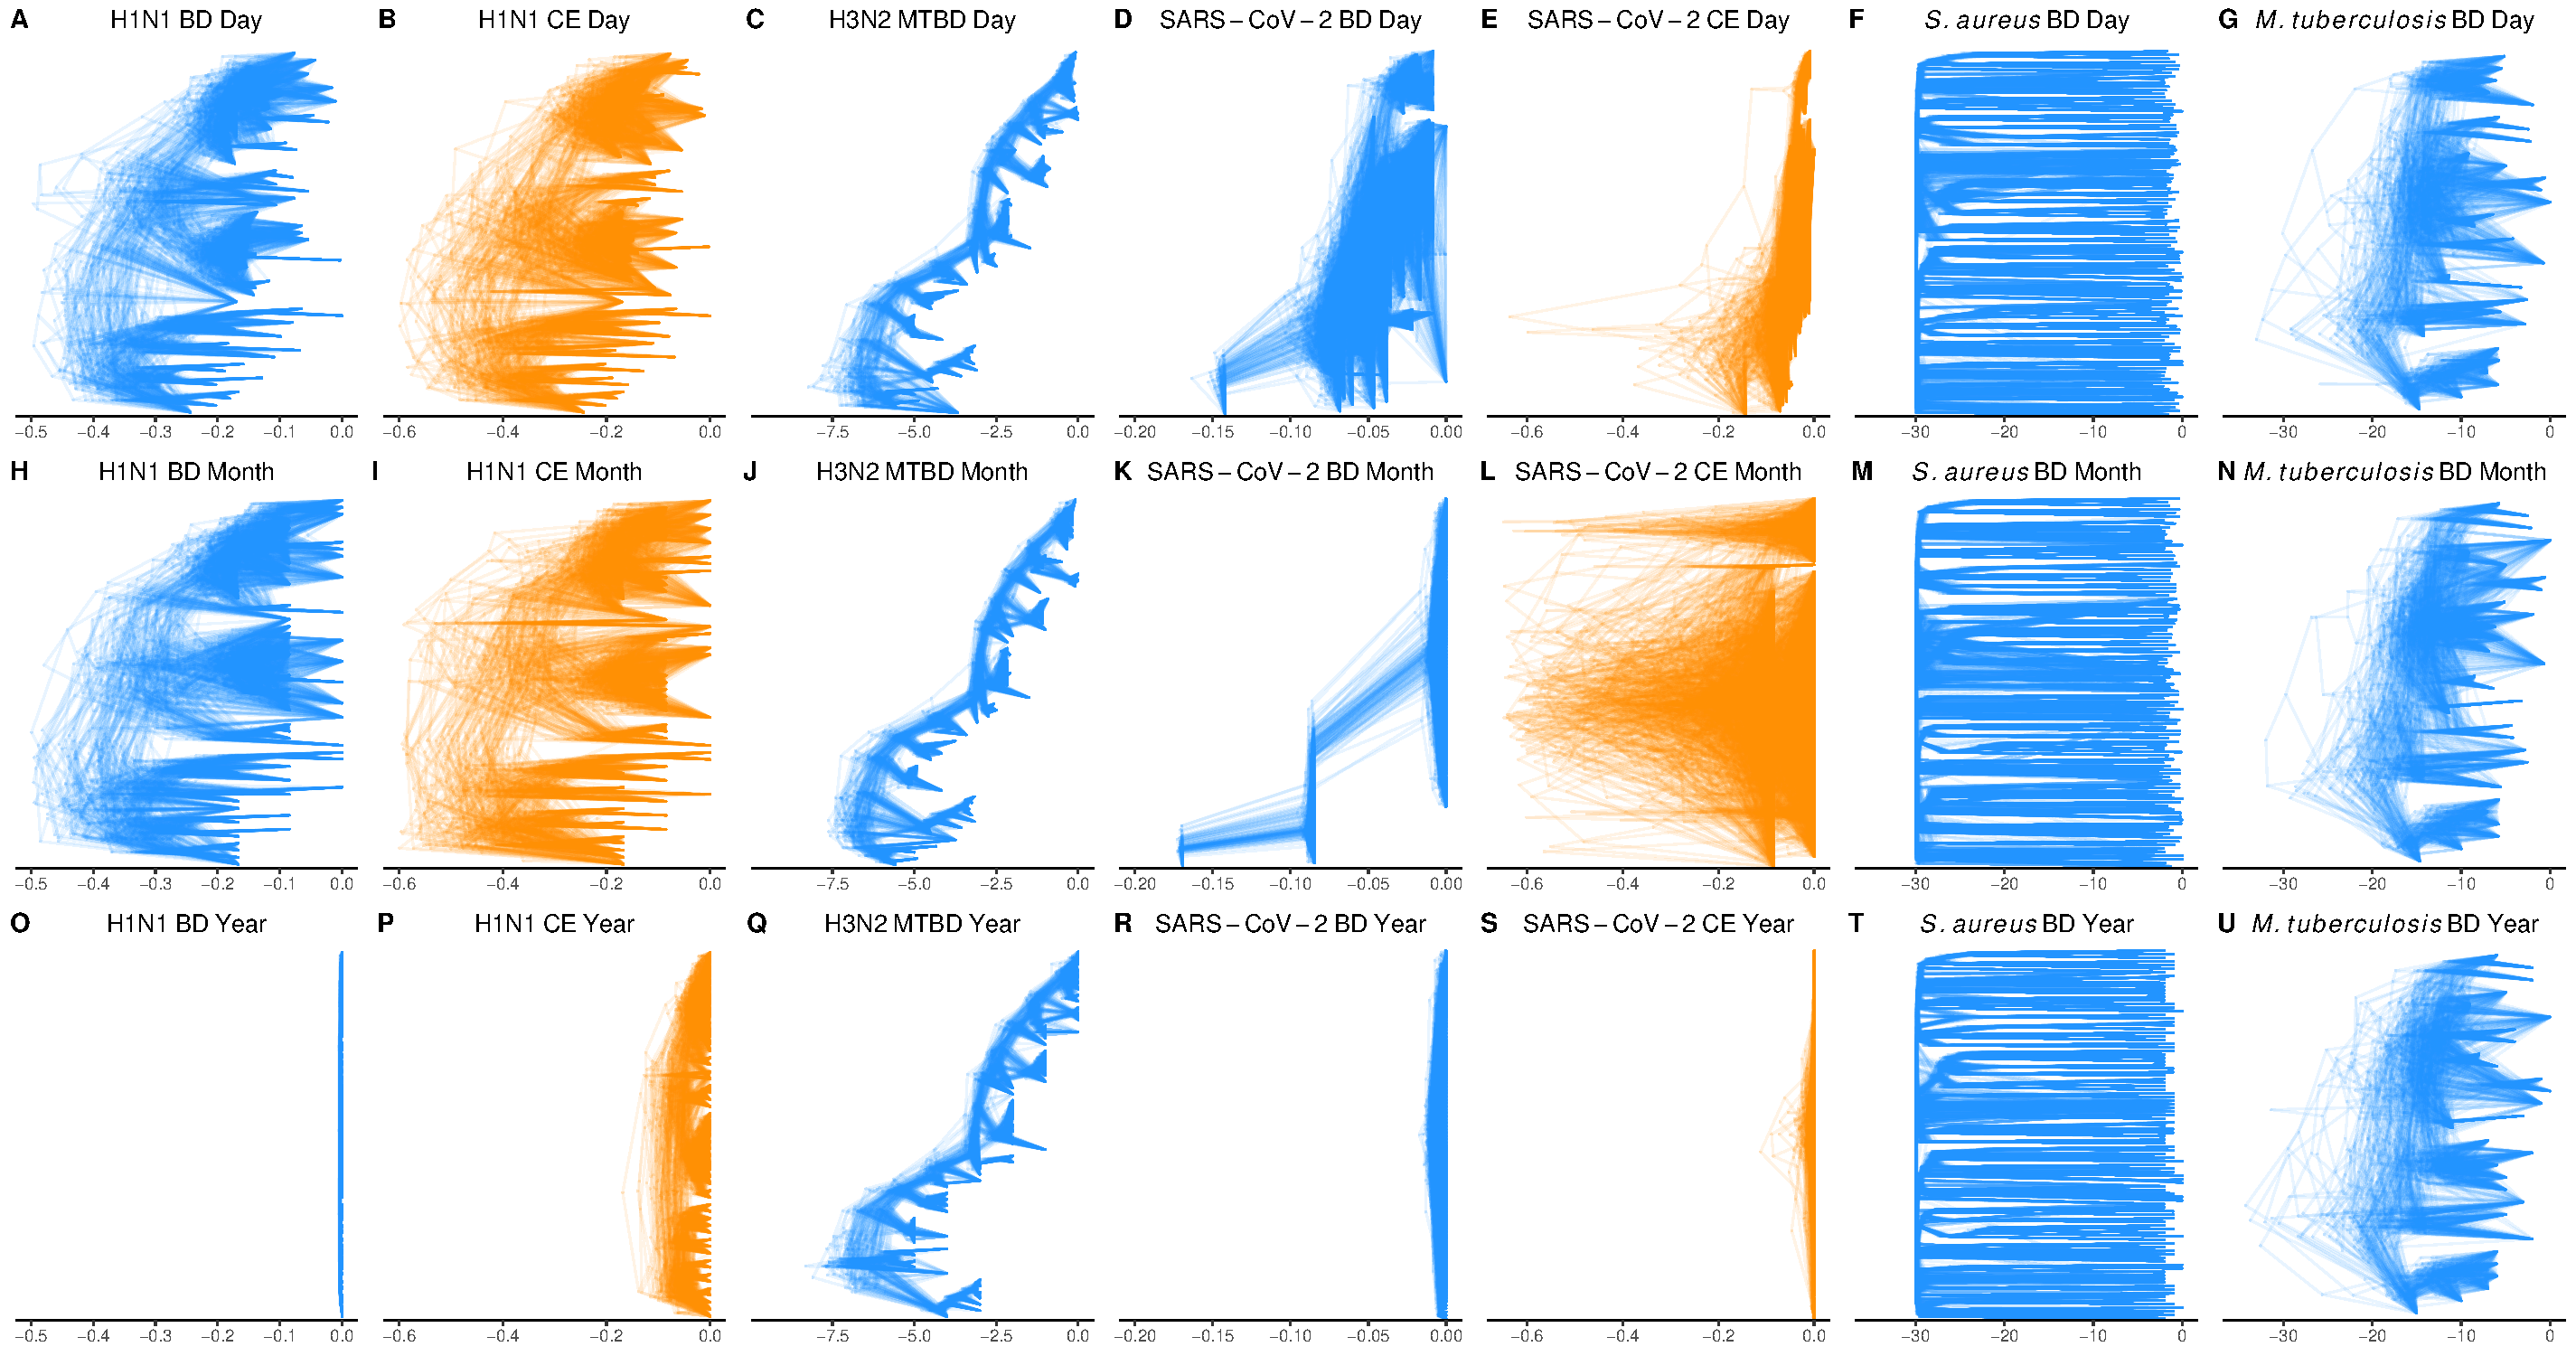
\includegraphics[width=\textwidth]{empirical_densitrees.pdf}
    \caption{Desnsitrees (overlayed posterior trees) for empirical data with columns corresponding to pathogen under each combination of date resolution and tree prior. For the H1N1 and SARS-CoV-2 treatments, Year resolution causes trees to collapse to instantaneous bursts.}
    \label{fig:densitree}
\end{figure}

\begin{figure}
    \centering
    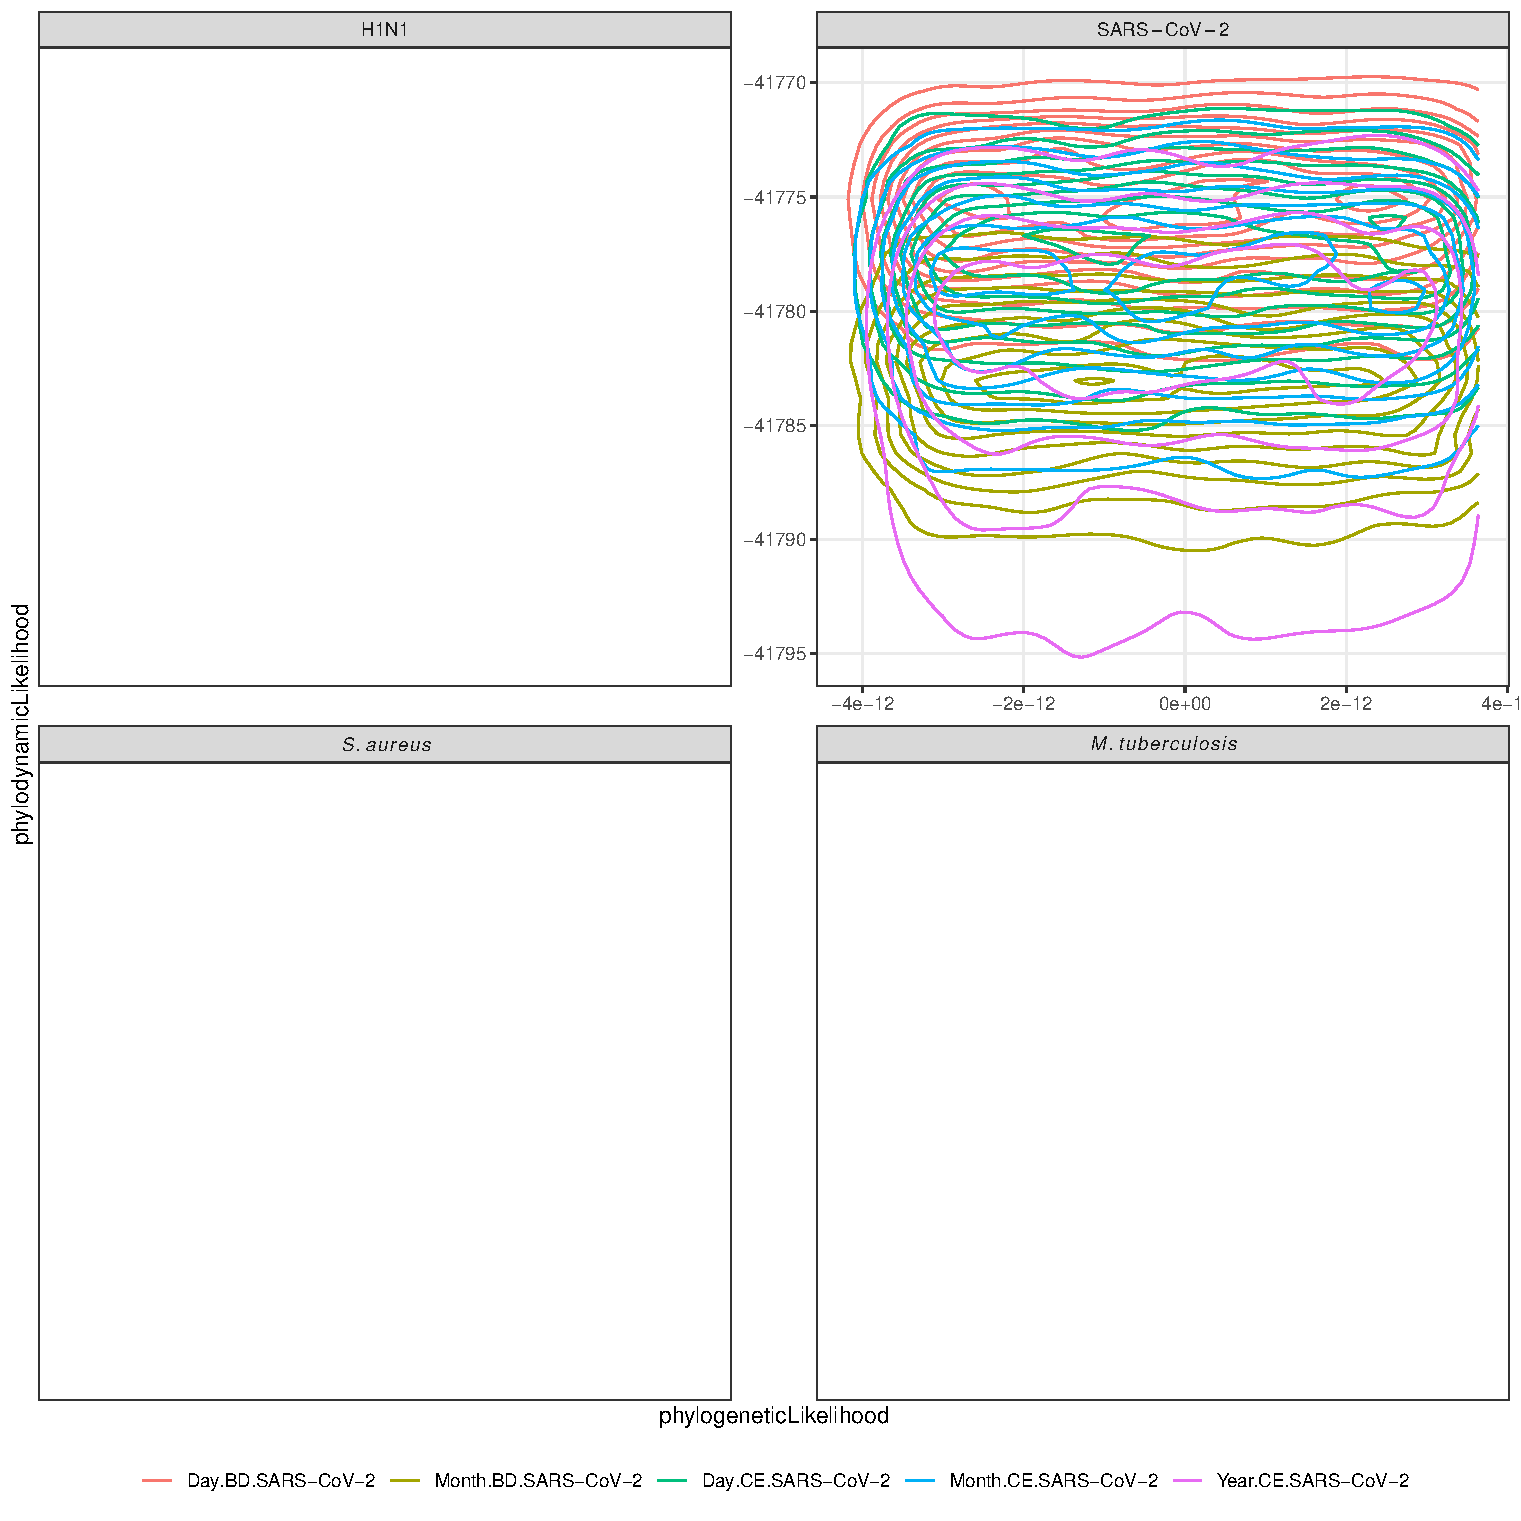
\includegraphics[width=\textwidth]{simulation_likelihood.pdf}
    \caption{Adjusted phylodynamic likelihood against adjusted phylogenetic likelihood with panels corresponding to each simulation condition. Points correspond to mean posterior likelihood for each simulated dataset under each simulation condition. Colour corresponds to date resolution. Likelihoods are adjusted by subtracting the mean phylodynamic or phylogenetic likelihood at Day resolution from each the means under Month and year resolution. Resulting points therefore show the difference phylodynamic and phylogenetic likelihoods due to date rounding with the point $(0, 0)$ representing likelihood at day resolution for each dataset. Month resolution generally results in smaller differences that Year resolution, suggesting coarser date resolution results in more perturbed likelihoods. There is also generally more error in phylodynamic likelihood than phylogenetic likelihood.}
    \label{fig:sim-likeihood}
\end{figure}


\begin{table}[]
    \centering
    \caption{Mean posterior estimates of substitution rate and outbreak age for empirical data with 95\% HPD in brackets.}
    \begin{tabular}{lccc}
        \toprule
         & Tree Prior & Substitution Rate (subs/site/yr) & Outbreak Age\\
        \midrule
        H1N1 & BD & 4.3e-3 (3.7e-3, 4.9e-3) & 3.7e-1 (3.3e-1, 4.2e-1)\\
        H1N1 & BD & 3.9e-3 (3.2e-3, 4.6e-3) & 3.5e-1 (3.1e-1, 4.1e-1)\\
        \addlinespace
        H1N1 & CE & 3.9e-3 (3.2e-3, 4.5e-3) & 4.2e-1 (3.6e-1, 5.0e-1)\\
        H1N1 & CE & 3.2e-3 (2.6e-3, 3.8e-3) & 4.6e-1 (3.8e-1, 5.6e-1)\\
        \addlinespace
        SARS-CoV-2 & BD & 2.5e-4 (1.1e-4, 4.5e-4) & 1.4e-1 (1.4e-1, 1.5e-1)\\
        SARS-CoV-2 & BD & 6.6e-4 (3.3e-4, 1.1e-3) & 1.7e-1 (1.7e-1, 1.7e-1)\\
        \addlinespace
        SARS-CoV-2 & CE & 2.4e-4 (9.1e-5, 4.7e-4) & 2e-1 (1.4e-1, 3.6e-1)\\
        SARS-CoV-2 & CE & 4.3e-5 (4.4e-6, 1.4e-4) & 1.6 (2.9e-1, 5.9)\\
        \addlinespace
        \textit{S. aureus} & BD & 1e-5 (1e-5, 1e-5) & 3e+01 (3e+01, 3e+01)\\
        \textit{S. aureus} & BD & 1e-5 (1e-5, 1e-5) & 3e+01 (3e+01, 3e+01)\\
        \textit{S. aureus} & BD & 1e-5 (1e-5, 1e-5) & 3e+01 (3e+01, 3e+01)\\
        \addlinespace
        \textit{M. tuberculosis} & BD & 1e-7 (6.5e-8, 1.4e-7) & 2.2e+01 (1.7e+01, 3.2e+01)\\
        \textit{M. tuberculosis} & BD & 1e-7 (6.6e-8, 1.4e-7) & 2.2e+01 (1.7e+01, 3.2e+01)\\
        \textit{M. tuberculosis} & BD & 9.9e-8 (6.2e-8, 1.4e-7) & 2.2e+01 (1.8e+01, 3.4e+01)\\
        \bottomrule
    \end{tabular}

    \label{tab:emp-clock-age}
\end{table}

\begin{table}[]
    \centering
    \caption{Mean posterior estimates of $R_{\bullet}$ for empirical data with 95\% HPD in brackets.}
    \begin{tabular}{lcccc}
    \toprule
     & Tree Prior & $R_0$ & $R_{e_1}$ & $R_{e_2}$\\
    \midrule
    H1N1 & BD & 1.1 (1.1, 1.1) & - & -\\
    H1N1 & BD & 1.1 (1.1, 1.2) & - & -\\
    \addlinespace
    H1N1 & CE & 1.1 (1.1, 1.2) & - & -\\
    H1N1 & CE & 1.1 (1.1, 1.2) & - & -\\
    \addlinespace
    SARS-CoV-2 & BD & 1.2 (9.3e-1, 1.6) & - & -\\
    SARS-CoV-2 & BD & 5.8 (3.7, 9.0) & - & -\\
    \addlinespace
    SARS-CoV-2 & CE & 1 (9.6e-1, 1.0) & - & -\\
    SARS-CoV-2 & CE & 1 (9.8e-1, 1.1) & - & -\\
    \addlinespace
    \textit{S. aureus} & BD & - & 1.6 (1.5, 1.7) & 6.6e-1 (5.1e-1, 8.0e-1)\\
    \textit{S. aureus} & BD & - & 1.6 (1.5, 1.7) & 6.8e-1 (5.4e-1, 8.3e-1)\\
    \textit{S. aureus} & BD & - & 1.7 (1.6, 1.8) & 3.7e-1 (1.9e-1, 5.4e-1)\\
    \addlinespace
    \textit{M. tuberculosis} & BD & - & 2.8 (5.8e-1, 5.3) & 1.4 (7.2e-1, 2.7)\\
    \textit{M. tuberculosis} & BD & - & 2.7 (5.7e-1, 5.0) & 1.4 (7.4e-1, 2.7)\\
    \textit{M. tuberculosis} & BD & - & 2.7 (4.6e-1, 5.1) & 1.5 (8.1e-1, 2.9)\\
    \bottomrule
    \end{tabular}

    \label{tab:emp-re}
\end{table}


\end{document}